\documentclass{article}
%=================================================
% Basics
%=================================================
\usepackage{fixltx2e} % Makes \( \) equation style robust, among other
                      % things. Must be the first package.


% Makes ligatured fonts searchable and copyable in pdf readers
\usepackage{cmap} % Load before fontenc 

% Always include these font encodings in your document 
% unless you have a very good reason.
\usepackage[T1]{fontenc}
\usepackage[utf8]{inputenc}

\usepackage{verbatim}

%=============
% Fonts
%=============

\usepackage{lmodern} % Improved version of computer modern
\usepackage[scale=0.88]{tgheros} % Helvetica clone for sans serif font


\newcommand\hmmax{2} % Default is 3.
\newcommand\bmmax{2} % Default is 4.

\usepackage{bm} % boldmath must be called after the package
\providecommand{\mathbold}[1]{\bm{#1}}

%=============
% AMS Packages and fonts
%=============
\usepackage{amsmath,amsbsy,amsgen,amscd,amsthm,amsfonts,amssymb} 

%=============
% Margins and paper size
%=============
\usepackage[centering,top=1.5in,bottom=1.2in,left=1.4in,right=1.4in]{geometry}
\usepackage{parskip}


%=============
% Section headings
%=============
\usepackage[sf,bf,compact]{titlesec}

%=============
% Tables and lists
%=============
\usepackage{booktabs,longtable,tabu} % Nice tables
\setlength{\tabulinesep}{1mm}
\usepackage[font=small,margin=10pt,labelfont={sf,bf},labelsep={space}]{caption}

%=============
% Code output
%=============
% \usepackage{listings}
% \usepackage{minted}




\usepackage{enumitem}
\setitemize{itemsep=0pt} 
\setenumerate{itemsep=0pt}
\setlist{labelindent=\parindent,%  % Recommended by enumitem package
  font=\sffamily}


%=============
% Hyperlink colors
%=============
\usepackage[usenames,dvipsnames]{xcolor}
\definecolor{steelblue}{HTML}{A1BDC7}
\definecolor{orange}{HTML}{D98C21}
\definecolor{silver}{HTML}{B0ABA8}
\definecolor{rust}{HTML}{B8420F}
\definecolor{seagreen}{HTML}{2E6B69}
\definecolor{joshua}{HTML}{FBDC7F}
\definecolor{darksky}{HTML}{154c79}

\colorlet{steelblue}{silver!30!white}
\colorlet{darkorange}{orange!85!black}
\colorlet{darksilver}{silver!85!black}
\colorlet{darksteelblue}{steelblue!85!black}
\colorlet{darkrust}{rust!85!black}
\colorlet{darkseagreen}{seagreen!85!black}

\usepackage{url}
\usepackage[colorlinks=true]{hyperref}
\hypersetup{linkcolor=darkrust}    
\hypersetup{citecolor=darkseagreen}      
\hypersetup{urlcolor=darksilver}     

%=============
% Microtype
%=============
\usepackage[final]{microtype} 

%=====================
% Header
%=====================
% \usepackage{fancyhdr}
% \usepackage{nopageno} % Gets rid of page number at the bottom
% \fancyhf{} % Clear header style
% \renewcommand{\headrulewidth}{0.5pt} % remove the header rule
% \pagestyle{fancy}
% \fancyhead[LE,RO]{\textsf{\small \thepage}}
% 
% \setlength{\headheight}{14pt}
%=====================
% Fix delimiters
%=====================

% Fixes \left and \right spacing issues. See discussion at
% http://tex.stackexchange.com/questions/2607/spacing-around-left-and-right
\let\originalleft\left
\let\originalright\right
\renewcommand{\left}{\mathopen{}\mathclose\bgroup\originalleft}
\renewcommand{\right}{\aftergroup\egroup\originalright}

%=================================================
% Math macros
%=================================================

%=============
% Generalities
%=============
\usepackage{mathtools}
\mathtoolsset{centercolon}  % Makes := typeset correctly for definitions

%%% Equation numbering
%\numberwithin{equation}{section} 

%%% Annotations
\newcommand{\notate}[1]{\textcolor{red}{\textbf{[#1]}}}

%==============
% Symbols
%==============
\let\oldphi\phi
\let\oldeps\epsilon

\renewcommand{\phi}{\varphi}
\renewcommand{\epsilon}{\varepsilon}
\newcommand{\eps}{\varepsilon}

%==============
% Constants
%==============

% Set constants upright
\newcommand{\cnst}[1]{\mathrm{#1}}  
\newcommand{\econst}{\mathrm{e}}

\newcommand{\zerovct}{\vct{0}} % Zero vector
\newcommand{\Id}{\mathbf{I}} % Identity matrix
\newcommand{\onemtx}{\bm{1}}
\newcommand{\zeromtx}{\bm{0}}

%==============
% Sets
%==============
\providecommand{\mathbbm}{\mathbb} % In case we don't load bbm

% Reals, complex, naturals
\newcommand{\R}{\mathbbm{R}}
\newcommand{\C}{\mathbbm{C}}
\newcommand{\K}{\mathbbm{K}}
\newcommand{\N}{\mathbbm{N}}

%==============
% Probability
%==============
\newcommand{\Prob}{\operatorname{\mathbbm{P}}}
\newcommand{\Expect}{\operatorname{\mathbb{E}}}

%==============
% Vectors and matrices 
%==============
\newcommand{\vct}[1]{\mathbold{#1}}
\newcommand{\mtx}[1]{\mathbold{#1}}

\newcommand{\mrange}{\operatorname{range}}
\newcommand{\mnull}{\operatorname{null}}



\DeclarePairedDelimiter{\ceil}{\lceil}{\rceil}
\DeclarePairedDelimiter{\floor}{\lfloor}{\rfloor}

\begin{document}

\title{CSE 6220 Homework 4}
\author{Karl Hiner, @khiner6}
\date{}
\maketitle

\section{}
Consider the following modification to the \textit{Sample Sort} algorithm described in class.
Suppose instead of choosing $p - 1$ local splitters per processor we choose $kp - 1$ local splitters per processor.
Prove that this modification guarantees the number of elements received by any processor is bounded by $\frac{n}{p}\left(1 + \frac{1}{k}\right)$.

\quad We can calculate the maximum number of elements received by any single processor by observing that the elements received will necessarily contain local splitters originating from other processors $P_i$.

The \textit{total} number of local splitters contained in the elements received by each processor will be $kp - 1$.
Since each processor contains $\frac{n}{p}$ elements, each local split will subdivide
$$\dfrac{\frac{n}{p}}{kp - 1} = \dfrac{n}{p}\cdot\dfrac{1}{kp - 1}$$
elements.
Thus, if a processor receives $s_i$ local splitters that originally came from $P_i$, we can bound the number of received elements $E_i$ that originated in $P_i$ by
$$E_i < \left(s_i + 1\right)\left(\dfrac{n}{p}\cdot\dfrac{1}{kp - 1}\right).$$ 
Finally, the total number of elements $E$ received by any processor will be bounded by
\begin{align*}
  E &< \sum\limits_{i=0}^{p-1}\left(s_i + 1\right)\left(\dfrac{n}{p}\cdot\dfrac{1}{kp - 1}\right)\\
  &= \left(\sum\limits_{i=0}^{p-1}\left(s_i + 1\right)\right)\left(\dfrac{n}{p}\cdot\dfrac{1}{kp - 1}\right)&\text{(separate terms w/o $i$)}\\
  &= \left(\sum\limits_{i=0}^{p-1}s_i + p\right)\left(\dfrac{n}{p}\cdot\dfrac{1}{kp - 1}\right)&\text{(evaluate $+ 1$ in sum)}\\
  &= \left(kp - 1 + p\right)\left(\dfrac{n}{p}\cdot\dfrac{1}{kp - 1}\right)&\text{(by def. of $s_i$, $\sum\limits_{i = 0}^{p - 1}{s_i} = kp - 1$)}\\
  &= \dfrac{n}{p}\cdot\dfrac{kp - 1 + p}{kp - 1}&\text{(rearrange)}\\
  &= \dfrac{n}{p}\left(1 + \dfrac{p}{kp - 1}\right) \approx \dfrac{n}{p}\left(1 + \dfrac{p}{kp}\right) &\text{(neglecting the $-1$ in the denominator)}\\
  &< \dfrac{n}{p}\left(1+\dfrac{1}{k}\right).&\text{(QED)}
\end{align*}
\section{}
Show that a $p$-processor ring can be embedded into a $p$-processor array with load = 1 and dilation = 2. Specify the mapping function from ring to array that works for arbitrary values of $p$.

\quad For load = 1, we must not have multiple nodes in the ring (source) mapped to a single node in the array (target).
Since we are given that the source and target have the same number of nodes, having load = 1 implies that we must have a one-to-one mapping between nodes.

For dilation = 2, every edge in the ring must map to at most two edges in the array.
Put another way, we must be able to travel between any two nodes that were originally neighbors in the ring with at most two hops in the array.

We can achieve this by interleaving the first half of the ring's nodes with the \textit{reversed} second half of its nodes.
Then, the ring's first node will have a direct link to its last node, the second node will have a direct link to the second-to-last node, and so on.

Here is an example:
\begin{verbatim}
Ring:  0-1-2-3-4-5-6-7-8-9 (9-0)
Array: 0-9-1-8-2-7-3-6-4-5
\end{verbatim}
Here is the mapping $\verb|rtoa|$ from processor rank $r$ in the ring to its corresponding rank in the array:
$$\verb|rtoa|(r) = \begin{cases} 2r & \text{if $2r < p$}\\2(p - r) - 1 & \text{otherwise}\end{cases}$$
\section{}

A three dimensional torus of size $16 \times 16 \times 8$ is embedded in a 2048-processor parallel computer that can route hypercubic permutations.
\begin{enumerate}[label=(\alph*)]
  \item Determine rank of the processor to which (9,13,6) is mapped.
  \begin{align*}
    (9,13,6) &= \texttt{btog}(9_{10})\|\texttt{btog}(13_{10})\|\texttt{btog}(6_{10})\\
    &= \texttt{btog}(\texttt{1001}_2)\|\texttt{btog}(\texttt{1101}_2)\|\texttt{btog}(\texttt{110}_2)&\text{(using (4,4,3) bits)}\\
    &= \texttt{1101}\|\texttt{1011}\|\texttt{101}\\
    &= \texttt{11011011101}_2 = 1757_{10}
  \end{align*}
  Thus, processor (9,13,6) has hypercube rank 1757.
  \item What is the torus rank of processor 532?

    We first convert 532 to binary, and then split it into segments of lengths (4,4,3) to find the gray codes of the three dimensions. 
    $$532_{10} = \texttt{01000010100}_2 = \texttt{0100}\|\texttt{0010}\|\texttt{100},$$
    and so we have gray codes $x = \texttt{0100}$, $y = \texttt{0010}$, and $z = \texttt{100}$.
    \begin{align*}
    (\texttt{gtob}(x),\texttt{gtob}(y),\texttt{gtob}(z)) &= (\texttt{gtob}(\texttt{0100}),\texttt{gtob}(\texttt{0010}),\texttt{gtob}(\texttt{100}))\\
    &= (\texttt{0111}_2,\texttt{0011}_2,\texttt{111}_2)\\
    &= (7_{10},3_{10},7_{10}).
  \end{align*}
  Thus, the torus rank of processor 532 is (7,3,7).
\end{enumerate}

\section{}
Consider the embedding of a 16-leaf complete binary tree into a 16-node hypercube assuming only one tree level at a time is involved computationally.
Consider processor with rank 12 in the hypercube.
\begin{enumerate}[label=(\alph*)]
  \item Which levels of the tree does this processor participate in?

  Let $j$ denote the number of trailing zeros in the binary representation of the processor rank $r$.
  Then, the processor with rank $r$ participates in levels $\log{p}, \dots, \log{p} - j$.
  
  For $p = 16, j = \text{TrailingZeros}\left(\texttt{1100}\right) = 2$, we have
  \begin{align*}
    \log{p}, &\dots, \log{p} - j\\
    \log{16}, &\dots, \log{16} - 2\\
    4, &\dots, 4 - 2\\
    4, &3, 2.
  \end{align*}
  Thus, the processor with rank 12 participates in levels 4, 3, and 2.
  \item For each level above, compute the tree rank of the node, and the hypercube rank of its parent, left child, and right child.

  \begin{itemize}
    \item Level 4:
    \begin{itemize}
      \item \textbf{Tree rank: (4,12)}.
      The rank within the leaf level is the same as the rank of the processor in the hypercube.
      \item \textbf{Parent hypercube rank: 12}.
      With $k$ denoting the level, change $\left(\log{p} - k\right)^{th}$ bit to $0$.
      $\implies$ Zero $\left(4 - 4 = 0\right)^{th}$ bit, which is already $0$.
      \item \textbf{Left/right child hypercube ranks: Leaf nodes have no children.}
    \end{itemize}
    \item Level 3:
    \begin{itemize}
      \item \textbf{Tree rank: (3,6)}.
      Leading $k = 3$ bits of hypercube rank of $\texttt{1100}$ = $\texttt{110}_2 = 6_{10}$.
      \item \textbf{Parent hypercube rank: 12}.
      Zero bit $4 - 3 = 1$, which is already $0$.
      \item \textbf{Left/right child HC ranks: 12 and 13}.
      Left child is always self.
      For right child, change $\left(\log{p} - k - 1 = 4 - 3 - 1 = 0\right)^{th}$ bit to $1$. 
    \end{itemize}
    \item Level 2:
    \begin{itemize}
      \item \textbf{Tree rank: (2,3)}.
      Leading $k = 2$ bits of hypercube rank of $\texttt{1100}$ = $\texttt{11}_2 = 3_{10}$.
      \item \textbf{Parent hypercube rank: 8}.
      Zero bit $4 - 2 = 2$ of $\texttt{1100} \to \texttt{1000}_2 = 8_{10}$
      \item \textbf{Left/right child HC ranks: 12 and 14}.
      For right child, change bit $4 - 2 - 1 = 1$ to $1$: $\texttt{1100} \to \texttt{1110}_2 = 14_{10}$. 
    \end{itemize}
  \end{itemize}

\end{enumerate}

\section{}
A Binomial tree of height $d$, termed $B(d)$ is defined as follows:
If $d = 0$, then $B(0)$ is a single node.
Otherwise, $B(d)$ is constructed by taking two binomial trees of height $d - 1$ and making the root of one tree the child of the root of the other tree.
Show that $B(d)$ can be embedded in a $d$-dimensional hypercube.

\begin{figure}[htb]
  \begin{center}
  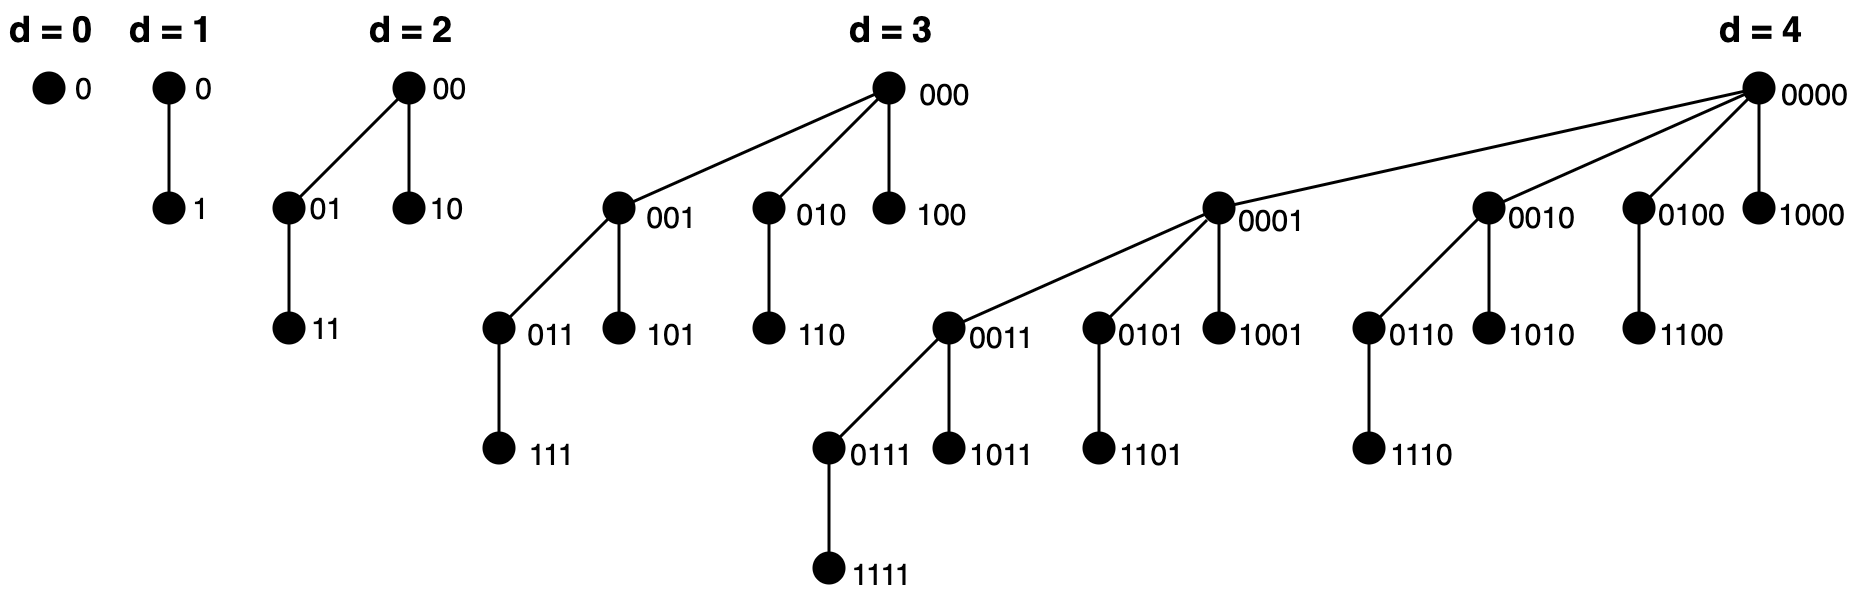
\includegraphics[width=110mm]{BinomialTreeEmbedding.png}
  \end{center}
\end{figure}

\quad Here is an algorithm for constructing a mapping from $B(D)$ to a $D$-dimensional hypercube:

\begin{itemize}
  \item \textbf{Construct $B(0)$:} $B(0)$ is a single rootnode, so we can embed it in a 0-dimensional hypercube by mapping the node to hypercube processor 0.
  \item \textbf{Iterate over $0 < d \leq D$:}
  \begin{itemize}
    \item Append $0$ to the binary representation of the hypercube rank of all nodes in $B(d - 1)$ until the length of the binary representation is $d$.
    (For $d = 1$, this is a no-op. For all other $d$, this is a left shift.)
    \item Create a copy of the tree with these $d$-dimensional ranks, add 1 to the ranks of all nodes in the copy, and add the resulting tree as a child of the root.
  \end{itemize}
\end{itemize}

\end{document}
